\documentclass[11pt,a4paper,titlepage]{article}
\usepackage[utf8]{inputenc}
\usepackage[english]{babel}
\usepackage[T1]{fontenc}
\usepackage{graphicx}
\usepackage{enumerate}

\title{Architectures of Intelligence \\ Homework 4}
\author{Ramon Meffert (S2702207) \\ Robin Koning (S2998254)}
\date{\today}


\begin{document}
\maketitle{}
\newpage

\section{(a)}
\label{sec:a}

\textbf{Show the learning of your model in a graph like the one
  above.}

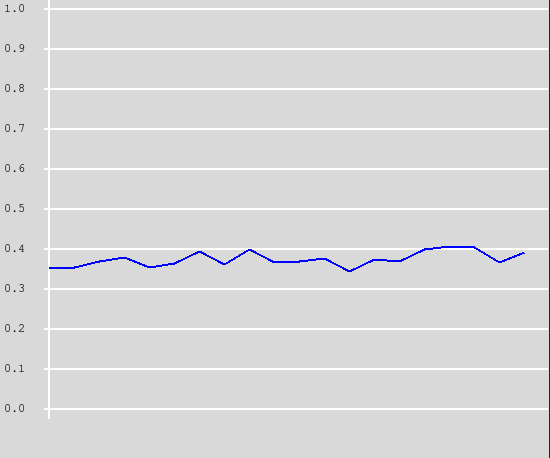
\includegraphics[scale=0.5]{learning-graph}

Textual representation of the image:
((0.3612 0.3776 0.3658 0.39300004)
 (0.351 0.355 0.368 0.379 0.353 0.365 0.395 0.362 0.4 0.366 0.368 0.376 0.344
  0.373 0.368 0.398 0.406 0.404 0.366 0.391))

\section{(b)}
\label{sec:b}

\textbf{Describe which information you store in memory, and explain
  why. Also indicate what information you use to retrieve a past
  experience.}
\\~\\
Information stored in memory:\\~\\
\begin{tabular}{@{$\bullet$}ll}
MC1 & First card our model gets.\\ 
MC2 & Second card our model gets.\\
MRESULT & Result of our hit/stay choice.\\
ACTION & The action belonging to that choice.\\
\end{tabular}
\\~\\
MC1 and MC2 are used to retrieve a more accurate (instead of just MC1)
game-state from DM.  MRESULT is used for debugging purposes to check
whether the model learns the correct action with a certain hand.
ACTION is saved to give the model a key to press if it remembers what
action it took previously with the same hand.
\\~\\
MC1 and MC2 are used to retrieve past experiences. This gives the
model some more information about the current state of the game than
just the first card and can be better used to determine the correct
action.
\section{(c)}
\label{sec:c}

\textbf{Describe how you changed the 'should-hit' and 'should-stay'
  productions, and explain why.}
\\~\\
For the 'should-hit' production: \\
The only additions to this production are that we now also check the
model's second card, and a test to determine whether the model should
actually hit or not. This test it simply a check whether the model's
total hand has a lower value than that of the opponent. If so, the
model is allowed to hit. This is a somewhat naive approach, but it is
sufficient to reach a point where the model wins ~39\% of the games
played.
\\~\\
For the 'should-stay' production: \\
The only addition to this production is that we now also save the
second card to our learned information.  This production did not need
a lot of modification, as it simply needs to get fired when the
model's total hand is greater than that of the opponent. This happens
because the should-hit production has a much higher utility function,
and would thus be fired first. Only when the should-hit production's
test fails (whether the model's total is lower than that of the
opponent's) should this production get fired.

\section{(d)}
\label{sec:d}

\textbf{Discuss whether this is a plausible model of playing black
  jack, and why/why not.}

This is a plausible model for playing black jack, after the model has
learned a lot of different hands, as the model emulates a simple
playing strategy, which is getting a higher total hand value
than that of the opponent.\\
This is similar to the way we normally play black jack, except for the
fact that we explicitly know not to exceed 21 points and can do simple
probability calculations to determine whether to hit or not is a good
choice.\\
The model however, does learn not to exceed 21 points implicitly,
thanks to the learned information about when to hit. But learning this
information implicitly takes a lot of hands to learn. \\
Thus the model is a plausible model for playing black jack, if it
learns a lot of information about what action to take with a certain
hand.

\end{document}

